\chapter{Model 3: Interacting Weyl Semimetal with two Weyl nodes}\label{chap:Model3}

So far, we have been discussing the gapping of the Dirac semimetal while preserving the \AFTR and $C_2$ symmetries. In this subsection, we focus on an opposite aspect of the symmetric many-body interaction -- the enabling of a (semi)metallic phase that is otherwise forbidden by symmetries in the single-body setting. We noticed in Subsec.~\ref{sec:anomaly} that the pair of momentum-separated Weyl points in Fig.~\ref{fig:Weylspectrum} is anomalous. In fact, it is well-known already that Weyl nodes~\cite{Murakami2007,WanVishwanathSavrasovPRB11,YangLuRan11,burkovBalenstPRL11,Ashvin_Weyl_review}, if separated in momentum space, must come in multiples of four in a lattice translation and time reversal symmetric three dimensional non-interacting system. 

This no go theorem can be rephrased into a feature. \begin{enumerate}\item If the low energy excitations of a \TR symmetric lattice (semi)metal in three dimensions consists of one pair of momentum-separated Weyl nodes, then the system must involve many-body interaction.\end{enumerate} We refer to this \TR and lattice translation symmetric strongly-correlated system as an interaction-enabled topological Dirac (semi)metal. We assume the Weyl nodes are fixed at two \TR invariant momenta, and therefore they are stable against symmetry-preserving deformations. Otherwise, if the Weyl nodes are not located at high symmetry points, they can be moved and pair annihilated. Also, as explained in the beginning of Sec.~\ref{sec:DiracSemimetal} and contrary to the more common contemporary terminology, we prefer to call the (semi)metal ``Dirac" rather than ``Weyl" because of the doubling. Perhaps more importantly, we propose the following conjecture. \begin{enumerate}\addtocounter{enumi}{1}\item Beginning with the interaction-enabled Dirac (semi)metal, {any} single-body symmetry-breaking mass must lead to a 3D gapped topological phase that cannot be adiabatically connected to a band insulator.\end{enumerate} We suspect this statement can be proven by a filling argument similar to that of Hasting-Oshikawa-Lieb-Schultz-Mattis~\cite{LiebSchultzMattis61,Oshikawa00,Hastings04}, and may already be available in Ref.~\cite{WatanabePoVishwanath17} by Watanabe, Po and Vishwanath. This conjecture applies to the coupled wire situation where the gapped phase is long-range entangled and supports fractional excitations. Its topological order is out of the scope of this article, but will be presented in a future work~\cite{SirotaRazaTeoappearsoon}. In a broader perspective, this type of statements may provide connections between strongly-interacting and non-interacting phases and help understanding quantum phase transitions of long-range entangled 3D phases from that of single-body band insulating ones.

Before discussing the three dimensional case, we make the connection to a few known interaction-enabled topological phases with or without an energy gap in low dimensions. First, zero energy Majorana fermions $\gamma_j=\gamma_j^\dagger$ in a true zero dimensional non-interacting (spinless) \TR symmetric system must bipartite into an equal number of positive chiral ones $\mathcal{T}\gamma_j\mathcal{T}^{-1}=+\gamma_j$ and negative chiral ones $\mathcal{T}\gamma_l\mathcal{T}^{-1}=-\gamma_l$. Fidkowski and Kitaev showed in Ref.~\cite{FidkowskiKitaev10} that under a combination of two-body interactions, eight Majoranas with the same chirality can acquire a \TR preserving mass and be removed from low energy. This leaves behind a collection of zero energy Majoranas that have a non-trivial net chirality of eight. Second, all $(1+1)$D \TR symmetric topological BDI superconductors~\cite{SchnyderRyuFurusakiLudwig08,Kitaevtable08,QiHughesRaghuZhang09,HasanKane10,QiZhangreview11,RMP} must break inversion because the zero energy Majorana boundary modes must have opposite chiralities at opposite ends. The Fidkowski-Kitaev interaction however allows one to construct a non-trivial $(1+1)$D topological model that preserves both \TR and inversion but at the same time supports four protected Majorana zero modes at each end~\cite{LapaTeoHughes14}. Third, a single massless Dirac fermion in $(2+1)$D is anomalous in a (spinful) \TR and charge $U(1)$ preserving non-interacting lattice system. On the other hand, it can be enabled by many-body interactions. For instance, when one of the two opposing surfaces of a topological insulator slab is gapped by symmetry-preserving interactions~\cite{WangPotterSenthilgapTI13,MetlitskiKaneFisher13b,ChenFidkowskiVishwanath14,BondersonNayakQi13}, a single massless Dirac fermion is left behind on the opposite surface as the only gapless low energy degrees of freedom of the quasi-$(2+1)$D system. Similar slab construction can be applied to the superconducting case, and interactions can allow any copies of massless Majorana fermions to manifest in $(2+1)$D with the presence of (spinful) \TR symmetry.

On the contrary, there are anomalous gapless fermionic states that cannot be enabled even by strong interactions. Chiral fermions that only propagate in a single direction cannot be realized in a true $(1+1)$D lattice system. They can only be supported as edge modes of $(2+1)$D topological phases such as quantum Hall states~\cite{Wenedgereview} or chiral $p_x+ip_y$ superconductors~\cite{Volovik99,ReadGreen}. Otherwise, they would allow heat transfer~\cite{KaneFisher97,Cappelli01,Kitaev06} from a low temperature reservoir to a high temperature one, thereby violating the second law of thermodynamics. Similarly, a single massless Weyl fermion can only be present as the $(3+1)$D boundary state of a $(4+1)$D topological bulk~\cite{ZhangHu01,BernevigChernHuToumbasZhang02,QiHughesZhang08,SchnyderRyuFurusakiLudwig08,Kitaevtable08}. It cannot exist in a true $(3+1)$D lattice system~\cite{Nielsen_Ninomiya_1981,NielsenNinomiyaPLB1981}, or otherwise under a magnetic field there would be unbalanced chiral fermions propagating along the field direction that constitute the ABJ-anomaly~\cite{Adler69,BellJackiw69,NielsenNinomiya83}.

\begin{figure}[htbp]
	\centering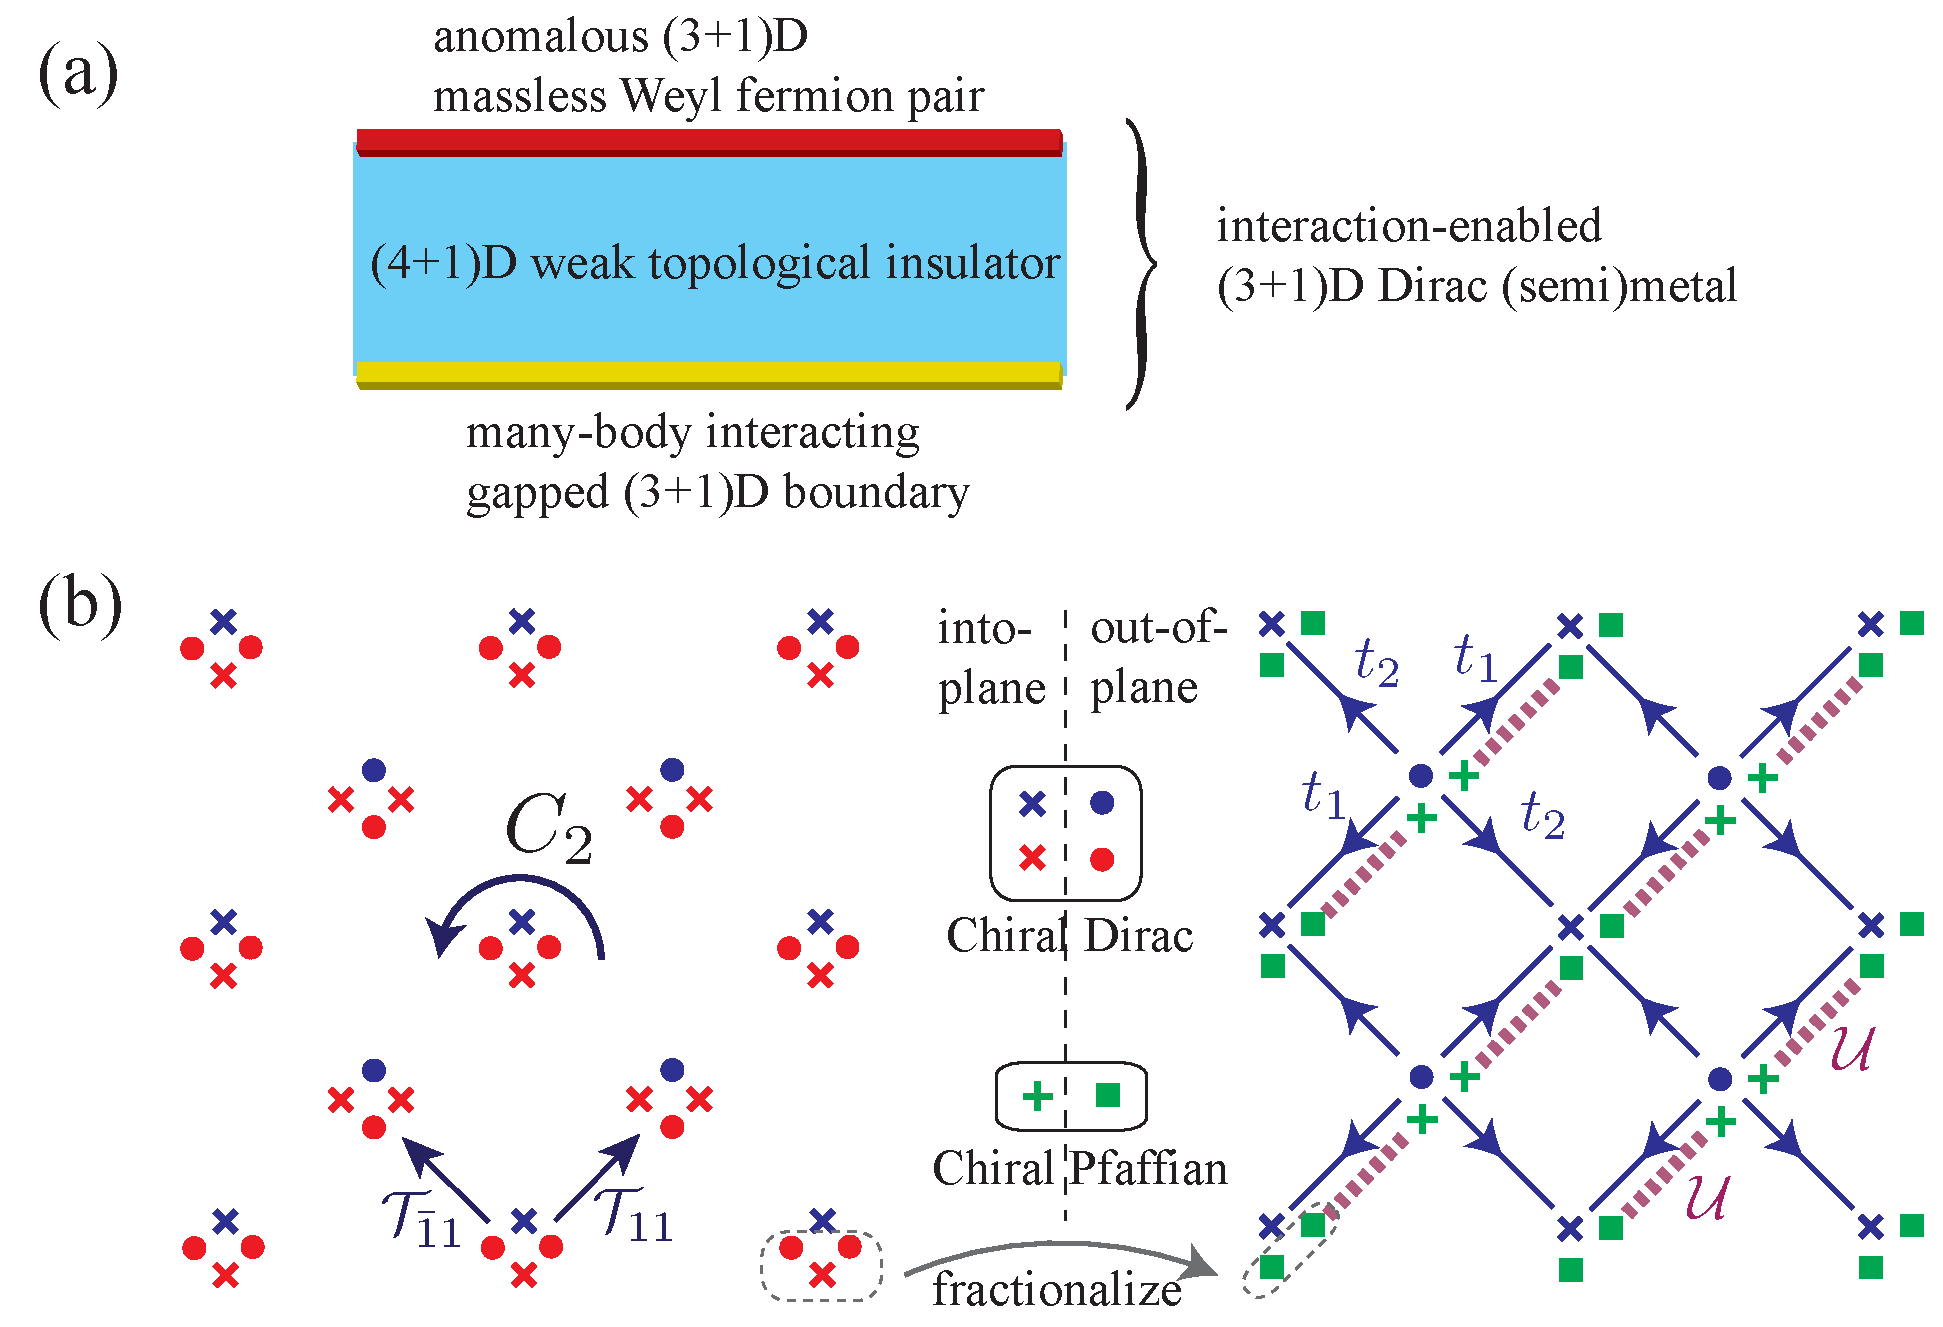
\includegraphics[width=0.94\textwidth]{intenable}
	\caption[(a) A quasi-$(3+1)$D interaction-enabled Dirac (semi)metal constructed by a 4D slab of WTI. (b) Coupled wire model of an anomalous Dirac (semi)metal.]{(a) A quasi-$(3+1)$D interaction-enabled Dirac (semi)metal constructed by a 4D slab of WTI. (b) Coupled wire model of an anomalous Dirac (semi)metal enabled by interaction with $C_2$ rotation and both AFTR $\mathcal{T}_{11},\mathcal{T}_{\bar{1}1}$ symmetries.}\label{fig:intenable}
\end{figure}

In this section, we focus on the simplest anomalous gapless fermionic states in $(3+1)$D that can be enabled by interactions. As eluded in Sec.~\ref{sec:holproj4D}, a weak topological insulator in $(4+1)$D can support the anomalous energy spectrum in Fig.~\ref{fig:Weylspectrum} on its boundary so that a pair of opposite Weyl points sit at two distinct \TRIM on the boundary Brillouin zone. A 4D \WTI slab, where the fourth spatial dimension is open and the other three are periodic, has two $(3+1)$D boundaries and each carries a pair of Weyl fermions. The coupling between the two pairs of Weyl fermions are suppressed by the system thickness and bulk energy gap. By introducing symmetry-preserving gapping interactions on the bottom surface, the anomalous gapless fermionic state is left behind on the top surface and is enabled in this quasi-$(3+1)$D setting (see Fig.~\ref{fig:intenable}(a)).

Inspired by this construction, we propose a true $(3+1)$D coupled wire model which has the anomalous energy spectrum in Fig.~\ref{fig:Weylspectrum} and preserves the \AFTR symmetries in both $\mathcal{T}_{11}$ and $\mathcal{T}_{\bar{1}1}$ directions as well as the $C_2$ (screw) rotation symmetry. The model is summarized in Fig.~\ref{fig:intenable}(b). It consists of a checkerboard array of electronic wires, where each wire has two chiral Dirac channels propagating into-paper and another two propagating out-of-paper. Contrary to the model considered in Sec.~\ref{sec:DiracSemimetal}, here the net chirality on each wire cancels and therefore the wires are true $(1+1)$D systems without being supported by a higher dimensional bulk. Using the splitting scheme described in Sec.~\ref{sec:gluing}, along each wire, one can fractionalize a group of three Dirac channels {\color{red}$\bullet\bullet\times$} ({\color{red}$\times\times\bullet$}) into a pair of co-propagating chiral Pfaffian channels {\color{green}$\blacksquare\blacksquare$} (resp.~{\color{green}$++$}). The two Pfaffian channels then can be backscattered in opposite directions using the many-body interaction $\mathcal{U}$ (dashed purple lines) described in Sec.~\ref{sec:interactionmodels}. This introduces an excitation energy gap that removes three Dirac channels per wire from low energy. Lastly, single-body backscatterings $t_1,t_2$ (solid directed blue lines) among the remaining Dirac channels {\color{blue}$\bullet\times$} described in \eqref{WeylTBHam} and Fig.~\ref{fig:WeylTB} give rise to the low-energy Weyl spectrum in Fig.~\ref{fig:Weylspectrum}. Since the many-body interaction $\mathcal{U}$ and the single-body backscatterings $t_1,t_2$ preserve the $C_2$ rotation and both \AFTR symmetries $\mathcal{T}_{11}$ and $\mathcal{T}_{\bar{1}1}$, the model describes an interaction-enabled anomalous (semi)metal that is otherwise forbidden in a non-interacting non-holographic setting. 

The non-local anti-ferromagnetic nature of the time reversal symmetry is built-in in the present coupled wire model. We speculate in passing that a local conventional \TR symmetric Dirac (semi)metallic phase consisting of a single pair of momentum-space-separated Weyl nodes may also be enabled by interaction. On one hand, the \AFTR symmetry could be restored to a local \TR symmetry by ``melting" the checkerboard wire array. On the other hand, there could also be an alternative wire configuration that facilitates a coupled wire model with a local conventional \TR symmetry.

Lastly, we gap the interaction-enabled Dirac semimetallic model (Fig.~\ref{fig:intenable}) by a symmetry-breaking single-body mass. This can be achieved by introducing electronic backscattering terms that dimerize the remaining Dirac channels {\color{blue}$\bullet\times$}, and were described by \eqref{DiracTBHam} in Sec.~\ref{sec:brokensymmetry}. The resulting state is an insulating $(3+1)$D topological phase with long-range entanglement. For instance, each diagonal layer gapped by the many-body interaction $\mathcal{U}$ has the identical topological order of the $\mathcal{T}$-Pfaffian surface state of a topological insulator. 

\section{Fractional Surface States}\label{sec:fracsurface}



In Sec.~\ref{sec:fermiarc1}, we discussed the surface states of the single-body coupled Dirac wire model \eqref{WeylTBHam} (see also Fig.~\ref{fig:WeylTB}). In particular, we showed in Fig.~\ref{fig:SurfaceStates1bdy} that an \AFTR symmetry preserving surface hosts open chiral Dirac channels, which connect and leak into the 3D (semi)metallic bulk. Earlier in this section, we discussed the effects of many-body interaction, which leads to two possible phases: (a) a gapped topological phase (see Sec.~\ref{sec:interactionmodels}) that preserves one of the two \AFTR symmetries, say $\mathcal{T}_{11}$, and (b) a gapless interaction-enabled Dirac semimetal (see Sec.~\ref{sec:intenable}) that preserves the $C_2$ rotation and both \AFTR symmetries $\mathcal{T}_{11}$ and $\mathcal{T}_{\bar{1}1}$. Here, we describe the boundary states of the two interacting phases on a surface closed under the symmetries.

\begin{figure}[htbp]
	\centering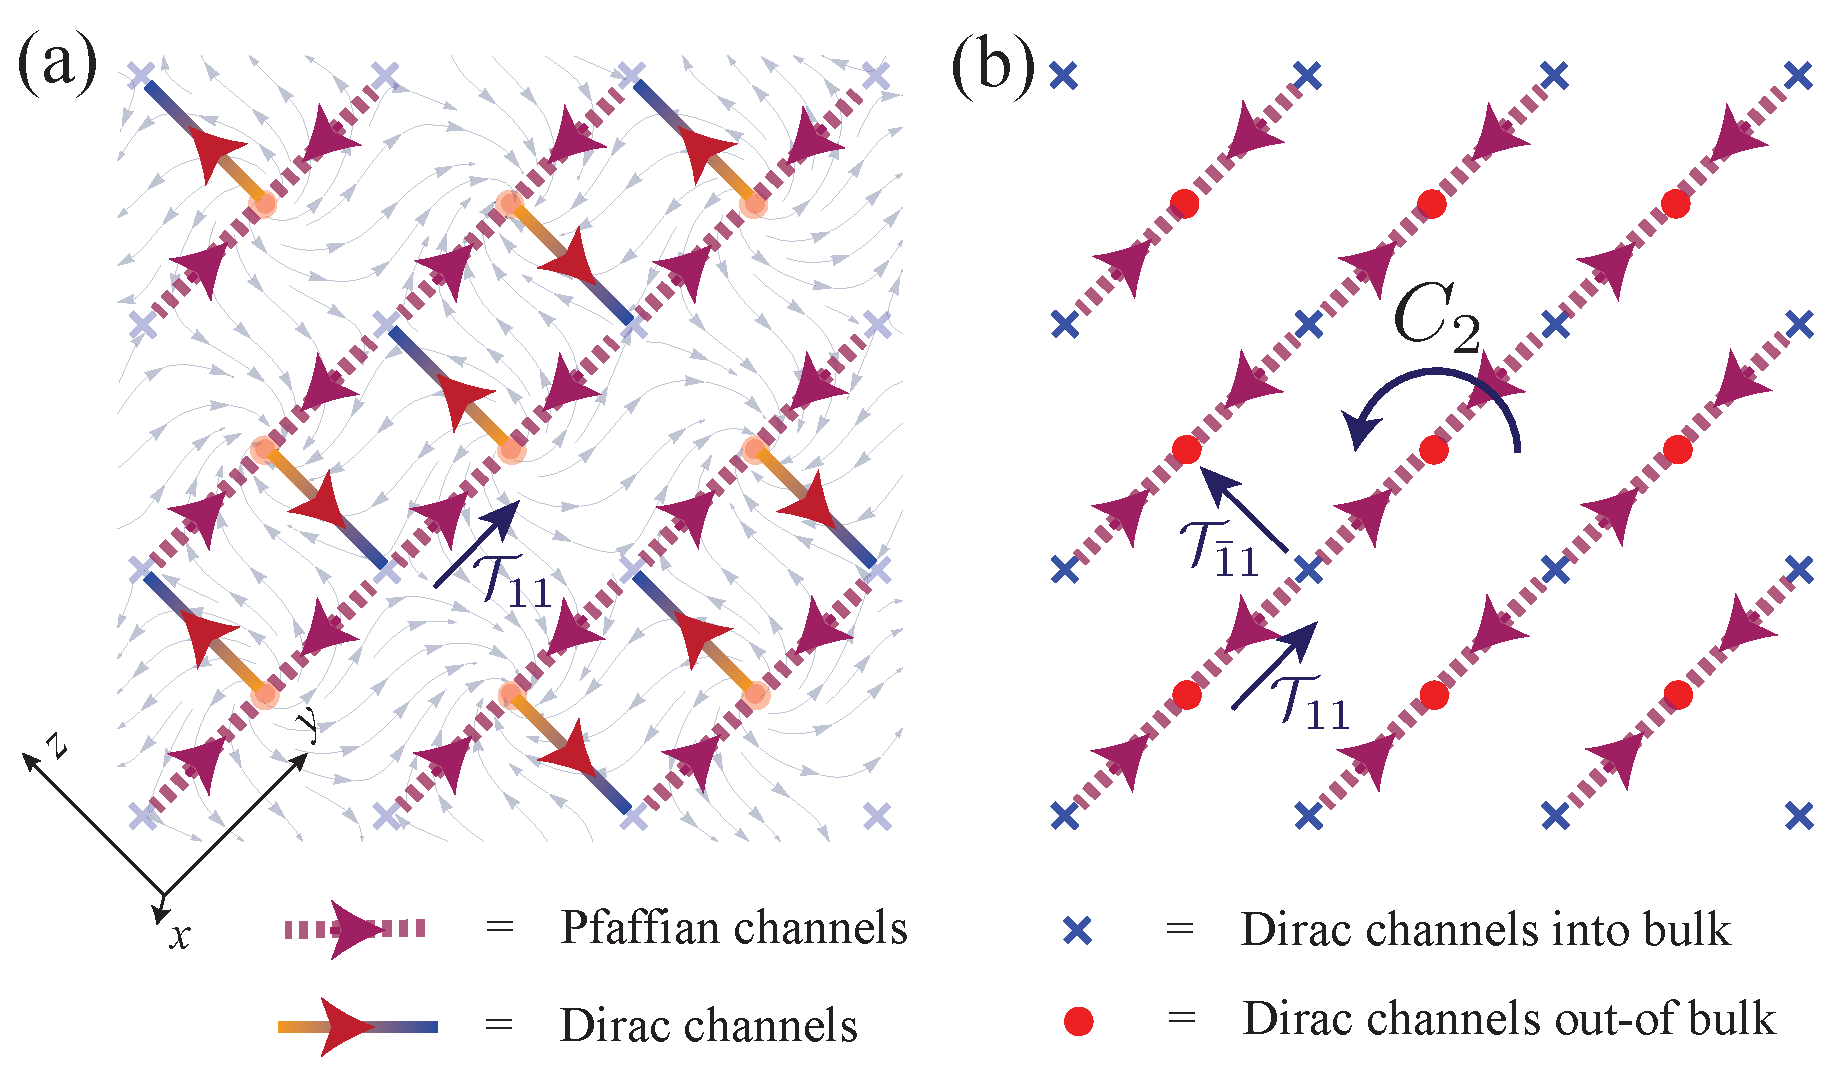
\includegraphics[width=0.96\textwidth]{SurfaceStates}
	\caption[Fractional surface states.]{Fractional surface states of (a) a 3D Dirac insulator gapped by many-body interaction that preserves $\mathcal{T}_{11}$, and (b) a 3D gapless interaction-enabled Dirac semimetal that preserves $\mathcal{T}_{11}$, $\mathcal{T}_{\bar{1}1}$ and $C_2$.}\label{fig:SurfaceStates}
\end{figure}

First, we consider the coupled wire model with the many-body interaction \eqref{mbdint} (see also Fig.~\ref{fig:gappinginteraction}) and a boundary surface along the $yz$-plane perpendicular to the wires. The surface network of fractional channels is shown in Fig.~\ref{fig:SurfaceStates}(a). We assume the bulk chiral Dirac wires ({\color{blue}$\times$}{\color{red}$\bullet$}) are supported as vortices of Dirac mass in the bulk (recall \eqref{DiracHam}), where the texture of the mass parameters is represented by the underlying vector field. The model is juxtaposed along the $yz$- boundary plane against the trivial Dirac insulating state $H_{\mathrm{vacuum}}=\hbar v{\bf k}\cdot\vec{s}\mu_z+m_0\mu_x$, which models the vacuum. The line segments on the surface plane where the Dirac mass $m_0\mu_x$ changes sign host chiral Dirac channels (c.f.~Subsec.~\ref{sec:fermiarcAFTRpreserving}).

Unlike the single-body (semi)metallic case in Fig.~\ref{fig:SurfaceStates1bdy} where the surface Dirac channels connects with the bulk ones, now the many-body interacting bulk is insulating and does not carry low-energy gapless excitations. Thus, the surface Dirac channels here cannot leak into the bulk and must dissipate to other low-energy degrees of freedom on the surface. The many-body interwire backscattering interaction in \eqref{mbdint} (and Fig.~\ref{fig:gappinginteraction}) leaves behind chiral Pfaffian channels on the surface. These fractional channels connect back to the surface Dirac channels in pairs. The surface network of chiral channels preserves the \AFTR $\mathcal{T}_{11}$ symmetry. However, the low-energy surface state is not protected. Electronic states can be localized by dimerizing the Pfaffian channels in the $z$ (or $\bar{1}1$) direction.

Second, we consider the interaction-enabled Dirac semimetallic model summarized in Fig.~\ref{fig:intenable}(b) in Sec.~\ref{sec:intenable} and again let it terminate along the symmetry preserving $yz$-plane perpendicular to the wires. The surface gapless channels are shown in Fig.~\ref{fig:SurfaceStates}(b). Here, the semimetallic bulk preserves $C_2$ as well as the two \AFTR symmetries $\mathcal{T}_{11}$ and $\mathcal{T}_{\bar{1}1}$. The bulk array of wires are true $(1+1)$D systems and are not supported as edge modes or vortices of a higher dimensional bulk. The pair of into-paper Dirac modes are bent into the pair of out-of-paper ones along each wire at the terminal. Similar to the previous case, the many-body bulk interwire backscattering interaction leaves behind surface chiral Pfaffian channels. Through the mode bending at the wire terminal, these Pfaffian channels join in pairs and connect to the chiral Dirac channels in the bulk that constitute the Dirac semimetal. In this case, the surface state is protected by $C_2$, $\mathcal{T}_{11}$ and $\mathcal{T}_{\bar{1}1}$, and is forced to carry fractional gapless excitations as a consequence and signature of the anomalous symmetries. For instance, the charge $e/4$ Ising-like quasiparticle and the charge $e/2$ semion can in principle be detected by shot noise tunneling experiments. These gapless fractional excitations however are localized on the surface because the Dirac (semi)metallic bulk only supports gapless electronic quasiparticles.